\subsection{Game Engine}
Game Enginen er skrevet i C\#, et objectorienteret programmering sprog
med stærkt library support der tillader udvikleren at fokusere på udvikling
af applikationer istedet for udvikling af libraries til at støtte projektet. \\

\noindent Nedstående præstenteres et diagram over de mest kritiske komponenter
Game Enginens interne spil logik og deres relationer til hinanden.
Der er ikke medtaget interfaces, eller klasser som er map, items, BackendController 
og logs som er mere specifikke til spillet og ikke til den interne logik.\\

\begin{figure}[H]
  \centering
   
  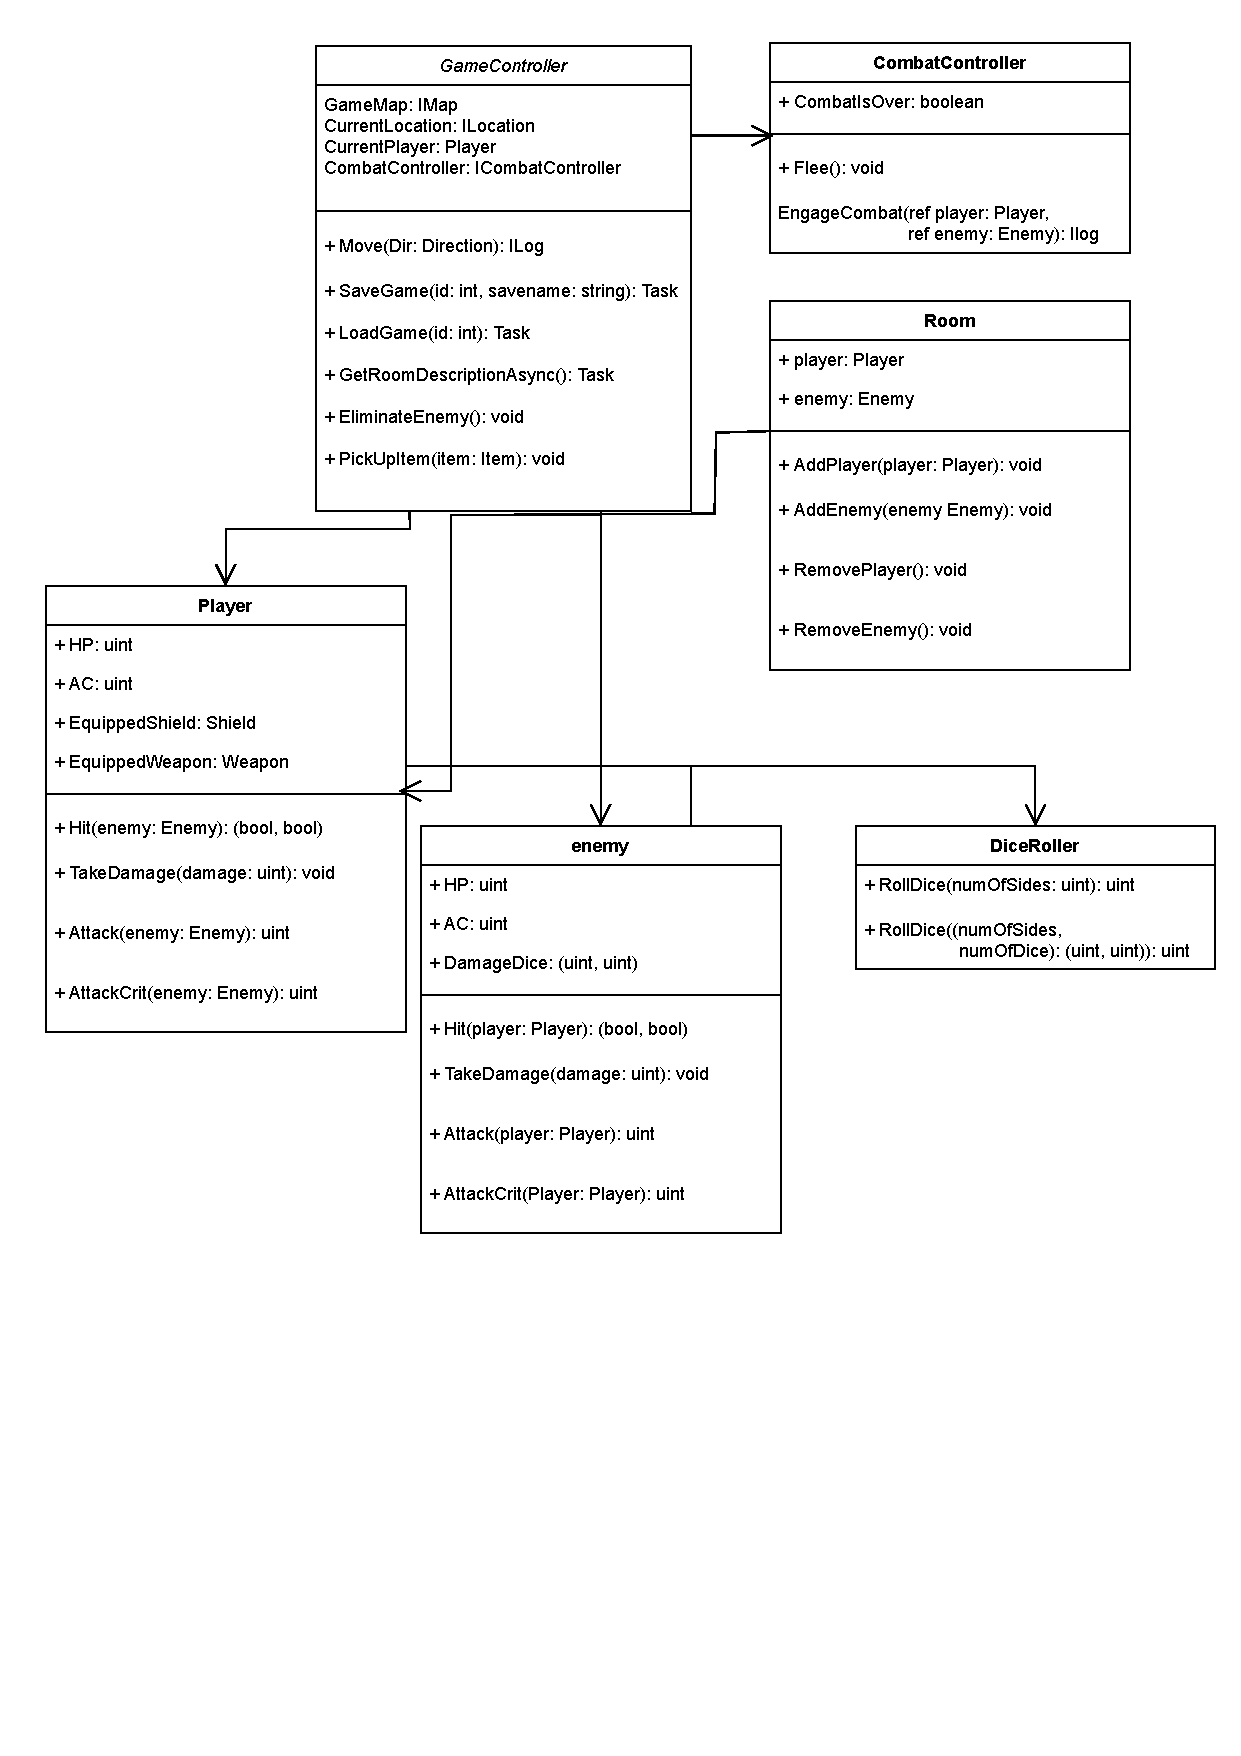
\includegraphics[width=0.9\linewidth, height=15cm, trim = 0 8cm 0 0cm]{02-Body/Implementering/GameEngineImplementering/Images/Core Class Diagram.pdf}
  \caption{Viser det mest definerende elementer af Game Engine og deres relationerne til hinanden. Der er her ikke medtaget interface,
           abstract klasser, item, logs og map. }%
  \label{fig:CoreClassDiagram}
\end{figure}

\subsubsection{Gamecontroller Implementering}

\noindent GameControlleren er det centrale komponent i game enginen, denne er ansvarlig 
for kommunikation til frontend del af applikationen. I denne implementering af 
GameControlleren har den adgang til alle spillet funktionaliteter gennem dennes
association til Combatcontroller, se \autoref{fig:CoreClassDiagram}, og BackendController
, som ikke er vist på \autoref{fig:CoreClassDiagram}.

Fra et implementering perspektiv er dette en nem løsning for en lille applikationen som denne
men fra et design perspektiv er dette en dårlig løsning. GameControlleren har alt for mange
grunde til at ændre sig og følger næppe SOLID principperne. \\

GameControlleren saver og loader spillet gennem sin relation til BackendController. 
Desværre er load funktionen ret kompliceret og burde være delt op i mindre functioner.
Source code for load kan ses på \autoref{fig:LoadFunction}

Koden bliver kompliceret idet den forsøger at gennemløbe alle Room objects i spillet
for på korrektvis at fjerne enemies og items, som allerede er blevet samlet op tidligere.
Her gennemløbes alle Room objects og i hvert room gennemløbes alle items i Room chest
objectet for at krydsreferer alle items med inventory listen for at se om de skal fjernes
som en del af save gamet.

Ligeledes håndtere den enemies og krydsreferer alle enemies med slainEnemies listen for at
se hvilke enemies spilleren allerede har besejret. Disse enemies fjerne herefter fra spillet.

\begin{figure}[H]
  \centering
  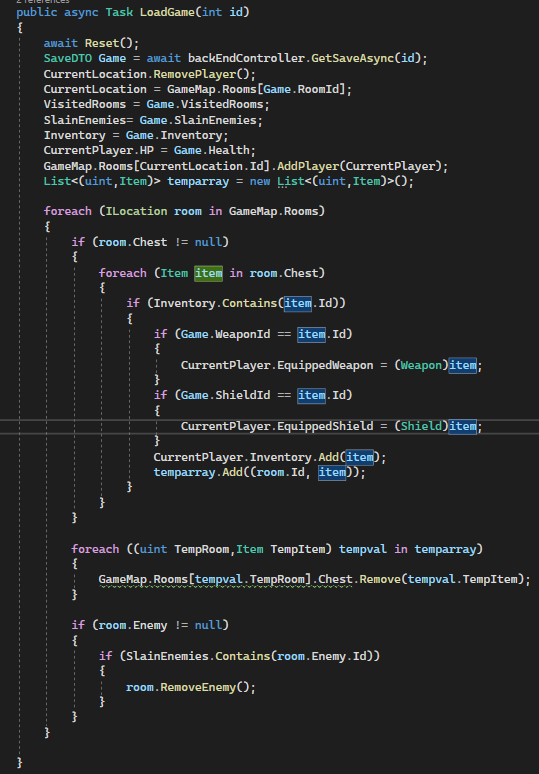
\includegraphics[]{02-Body/Implementering/GameEngineImplementering/Images/LoadFunction.png}
    \caption{Load funktionen, resetter game, setter de rigtige states og gennemløber
           alle Room instances og sætter deres state til den korrekte state.}
  \label{fig:LoadFunction}
\end{figure}



\subsubsection{Generering af Map}
\noindent Map klassen generer et map til spillet. Denne består af en
simple liste af lister over, hvilket rooms hvert room er 
forbundet til.

Denne Process er kompliceret og kræver en uddybende forklaring. Problemet 
består i at afgøre hvordan man sikre at det samme map bliver genereret
hver gang spillet loades. 

\paragraph{Gem en map layout fil \\}
Denne løsning viste sig at være den bedste løsning for at sikre sig, at 
map layoutet kun skulle eksistere i en enkel folder i projektet.
Men det viste sig vanskelig at læse en sådan fil uafhængigt af pc'en 
programmet blev kørt på.

\paragraph{Lav en klasse som generer map layout filen \\}
Ultimativt blev dette løsningen, som benyttes i projektet. En MapCreator
klasse danner en map layout fil når dens konstruktor bliver kald.

En map klasse som store map layoutet kan nu læse layout filen og 
danne et map udfra denne fil.
Filen består af linjer med formen \textit{``leftRoomId, TopRoomId, RightRoomId, BottomRoomId''}. Den først linje dækker room 1, næste linje dækker room 2 osv.

Hver linje i map layout filen mappes til en liste af roomId'er,  der kan insertes i Map
klassens mapLayout listea. Denne Liste danner grundlaget for spillets map og 
diktere hvordan spilleren kan navigere i spillet. Denne mapping mellem strings og int array
er vist i \autoref{fig:RoomConverter}.

\begin{figure}[h]
  \centering
  \caption{viser illustrer hvordan en linje fra map layout filen omdannes til en liste af room id'er 
           som rummet er forbundet med. Dette er kerne mekanismen for hvordan en spiller kan navigere
           rund i spillet, da en spiller ikke kan bevæge sig fra et Room til et anden, der ikke er 
           i denne liste af forbindelser mellem det nuværende room og den ønskede bevægelses retning.}
  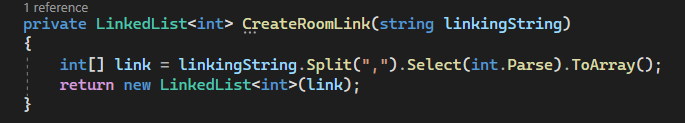
\includegraphics[scale=0.8]{02-Body/Implementering/GameEngineImplementering/Images/MappingRoomString.png}
  \label{fig:RoomConverter}
\end{figure}

\paragraph{Items og Enemies \\}
Som det sker for rooms, ligeledes sker der for enemies og items. MapCreator klassen
generer seperate filer for enemy positions og item lokationer. Map klassen 
kan herefter læse filen og mappe hver linje i filen til, en enemy eller item og 
placere det i det korrekte room.


\subsubsection{Log}
Komunikkation med frontend fra GameControlleren og CombatControlleren
gør brug af en log.
Logen består af et dictionary datastruktur som GameControlleren og 
CombatControlleren benytter til at logge vigtige infomation, som 
frontend kunne have brug for at vise til spilleren. \\

\noindent Dette kan være infomation om spillerens bevægelse fra
et Room til et andet. Det kan også være infomation omkring spillerens
eller enemies tilbageværende livsmængde osv. Dette isolere frontend 
fuldt fra Game Engine, da frontend ikke har andre accesspunkter til
infomation om hvad der sker i spillet. 

Derved opnår frontend seperation of respondsibility da frontend nu 
kun er ansvarlig for at display infomation som det er givet af game
enginen.

\newpage


\subsection{Kommentar til implementeringen}

Gennem udviklingen af Game Enginen er der brugt interfaces eller abstrakte 
klasser til implementering af alle funktionaliteter. Dette gør det både nemt
at teste implementeringerne samt at udvide spillet. Men for scopet af opgaven
er dette nok ``Overkill''. Det er godt at bruge, men for en applikation så 
lille som denne, der ikke kommer til at udvide sig er det nok for meget 
boilerplate kode. 




